\documentclass[a4paper,12pt] {article}

\usepackage[utf8]{inputenc}
\usepackage[english,russian]{babel}

\usepackage{geometry}
\geometry{left=3cm}
\geometry{right=1cm}
\geometry{top=2cm}
\geometry{bottom=2cm}
\linespread{1.3}


\def\htag#1{\#\textit{#1}}  % short alias for hashtags style

\usepackage{graphicx}
\graphicspath{{pic/}}
\DeclareGraphicsExtensions{.png,.jpg}

\newcommand{\tocsecindent}{\hspace{7mm}}


\begin{document}


\begin{titlepage}
		
\thispagestyle{empty}
		
  \begin{center}
  
   
   ПРАВИТЕЛЬСТВО РОССИЙСКОЙ ФЕДЕРАЦИИ \\
   
   \vspace{0.25cm}
   ФЕДЕРАЛЬНОЕ ГОСУДАРСТВЕННОЕ БЮДЖЕТНОЕ
   ОБРАЗОВАТЕЛЬНОЕ УЧРЕЖДЕНИЕ ВЫСШЕГО ОБРАЗОВАНИЯ 
   «САНКТ-ПЕТЕРБУРГСКИЙ ГОСУДАРСТВЕННЫЙ УНИВЕРСИТЕТ» 
   (СПбГУ)
   
   \vspace{0.25cm}
   Направление: Прикладные математика и физика
   
 
   \begin{figure}[h!]
   	\begin{center}
   		
\includegraphics[width=0.25\linewidth]{Gerb}
   	\end{center}
   \end{figure}


     \textbf{\Large Полуавтоматическое структурирование
     изображений в социальной сети с помощью 
     методов машинного обучения}
     
 \bigskip

\vfill

\begin{flushright}
    \footnotesize{
    Выполнил: студент 2-го курса магистратуры кафедры вычислительной физики, А. Р. Шабанов
    
    Руководитель: доцент кафедры вычислительной физики, к.ф.-м.н., А. С. Немнюгин
    
    Рецензент: разработчик интеллектуальных систем в ООО “Мэйл.ру”, А. А. Дзюба
    }
\end{flushright}

\end{center}

\vfill

\newlength{\ML}
\settowidth{\ML}{«\underline{\hspace{0.7cm}}» \underline{\hspace{2cm}}}


\begin{center}
    Санкт - Петербург \\
    2019
\end{center}

\end{titlepage}



\tableofcontents
\setcounter{page}{2}


\newpage
\indent
\indent
С каждым днем пользователи социальных сетей создают и потребляют все б\'{о}льшие
и б\'{о}льшие объемы информации, в том числе огромное количество фотографий.
Построение системы для быстрой и точной навигации в миллионах изображений
 --- не тривиальная задача. Одно из самых распространенных решений этой
 проблемы заключается в использовании тегов. Частный случай такого подхода ---
 использование хештегов в социальных сетях.


\indent
\textit{Хештег} --- это любое слово или фраза без пробелов, перед которой стоит 
символ \#, который называется \textit{диез} или \textit{решетка}, а в англоязычном 
варианте -- \textit{hash}, отсюда и название. Приведем несколько примеров:
\htag{masterwork}, \htag{spbu}, \#htag{lovesport}. Обычно в браузере или 
приложении хештег отображается как гипертекст, кликнув по которому можно 
получить список публикаций, снабженных таким же тегом.

\indent
Кроме простоты и удобства теги обладают еще одним полезным свойством 
-- они позволяют не думать об  иерархии структурируемой информации. 
Например, набор изображений можно разложить
по папкам, создав иерархию по датам, геолокациям или авторству. Причем в отдельных
случаях подобрать наиболее подходящую иерархию бывает затруднительно. Проблему
можно решить так: достаточно поставить несколько тегов для всех изображений,
а сами они могут храниться в плоской системе файлов.
Благодаря этому свойству тегирование используются  для рубрикации контента 
не только только онлайн, но и в оффлайн приложениях, например, 
просмоторщиках фотографий. 


\indent
Можно выделить две разновидности популярных хэштегов в социальных сетях.
Первые, используемые недолго и посвященные каким-то социальным явлениям
или событиям, например: \htag{elections2018}, \htag{metoo}. 
И вторые, широкораспространенные, но не связанные с новостной повесткой, 
например: \htag{sport}, \htag{cafe}; они и будут нас интересовать.
 Данная работа посвящена разработке интеллектуальной системы, 
подсказывающей пользователю релевантные хештеги к загружаемым фотографиям.
 Кроме того, с помощью такой системы можно решать и 
  \textquotedblleft обратную\textquotedblright  задачу -- определять,
уместно ли поставлены те или иные теги к заданным изображениям. 
Способность системы давать ответ на такой вопрос можно использовать для 
выявления злоупотреблений со стороны пользователей. Например, зачастую
 в рекламных целях продвигаемые публикации снабжают множеством популярных 
 тегов, не имеющих никакого отношения к публикуемой информации.
 
  
\addcontentsline{toc}{section}{\tocsecindent{Введение}}


\newpage
\section{Постановка задачи}

todo Рассказать про другие работы о тегах (например, на фликре).

\indent
\indent
Данная работа посвящена разработке интеллектуальной системы, 
подсказывающей пользователю релевантные и широкораспространенные
хештеги к загружаемым фотографиям.
Можно выделить две разновидности популярных хэштегов в социальных сетях.
Первые являются выражением чувств, эмоций и других абстрактных понятий,
например \htag{love}, \htag{friendship}, \htag{happy}. Вторые непосредственно
связаны с объектами, находящимися в кадре, например  
\htag{sport}, \htag{cafe}, \htag{nature}. 
Интуитивно понятно, что для второй разновидности
тегов предсказательная система, построенная на машинном зрении, будет
давать более точные результаты, чем для первой (но будет
иметь относительно узкую специализацию). Чтобы построить такую систему
нужен подходящий набор обучающих данных, но существующие датасеты, 
собранные из социальных сетей, не разделяют тренировочные примеры на те, 
где визуальный контент напрямую связан с целевыми классами, и те, где это не так.
В связи с чем возникла идея для данной задачи 
адаптировать датасет, изначально не размеченный
хэштегами, но имеющий аннотации, связанные с объектами,
находящимися в кадре. Кроме того, датасет должен быть относительно небольшим,
чтобы не требовать значительных 
вычислительных ресурсов; но при этом достаточно разнообразным, чтобы 
быть релевантным как можно большему количеству загружаемого контента.
В настоящей работе автор остановил свой выбор на датасете мест и локаций 
 \textit{SUN (Scene Understanding Dataset\cite{sundata} (SUN)}, 
 разметка которого после некоторой предобработки может быть отображена в популярные хэштеги.


\indent  
\textit{SUN} -- это набор изображений для каждого из которых выбрана одна
  из четырехсот локаций (сцен), вот несколько примеров:
  
  
\begin{itemize}
    \item \textit{baseball field}
    \item \textit{basketball court}
    \item \textit{ice shelf}
    \item \textit{forest}
    \item \textit{wind farm}
\end{itemize}


\indent
  Большинство названий локаций сами по себе не являются популярными 
  тегами из социальных сетей. Поэтому необходимо
  сопоставить их широко распространенным хэштегам (если это возможно):
  
  \begin{itemize}
      \item \textit{baseball field, basketball court}  $\rightarrow$ \htag{sport}
      \item \textit{ice shelf, forest} $\rightarrow$ \htag{nature}
      \item \textit{wind farm} $\rightarrow \times$ 
  \end{itemize}
  
  \indent
  Обученная на таких данных модель по окружению,
   обнаруженному на пользовательском фото,
  сможет подсказывать ему подходящий хэштег.
  
  
  
  \indent
  Ясно, что полученная модель будет корректно работать лишь для
  ограниченного (пусть и большого) домена фотографий. Следовательно, необходимо 
  обучить её распознавать не входящие в этот домен классы и
   не пытаться определить их категорию. Кроме того, в случае низкой уверенности
   в правильности предсказания так же лучше ничего не делать. 
    По мнению автора, гораздо предпочтительнее не 
   предложить пользователю подходящий хэштег, чем многократно предлагать 
   нерелевантные варианты.
   
   \indent
В качестве модели компьютерного зрения в работе 
используются глубокие сверточные
нейронные сети. Данный выбор обосновывается тем, что в последние
годы сверточные сети отлично зарекомендовали себя для решения задач, связанных
с обработкой изображений. Mожно привести в пример самый большой 
и известный
конкурс по классификации изображений \textit{ImageNet}\cite{imagenet},
который проводится ежегодно с 2010 года, при этом, начиная с 2012 года классические
решения ни разу не побеждали, уступив место нейронным сетям.


  \indent
Научная новизна работы определяется:
\begin{itemize}

    \item Адаптацией датасета \textit{SUN} для решения задачи о структурировании
    изображений в социальных сетях;
    
    \item Исследованием новых схем обучения неронных сетей, предложенных автором.
     (todo Обучить сегментатор на подсете, сделать псевдолейблинг, 
     посмотреть точность, 
    что-то вроде supervised atention)
    
\end{itemize}









\newpage
\section{Используемые инструменты}

\indent
\indent
\textbf{Программные средства}

\indent
В качестве языка программирования использовался
 \textit{Python 3.6.7} (сборка \textit{Anaconda}),
 в качестве среды разработки --- \textit{PyCharm Professional 2018.1},
 операционная система \textit{Ubuntu 16.04.4 LT}. Использованы
 следующие сторонние библиотеки для \textit{python}:


\begin{itemize}

    \item \textit{pytorch, torchvision} --- построение и обучение нейронных сетей
    \item \textit{tensorboardX} --- визуальное логирование процесса обучения 
    \item \textit{PIL, opencv, scikit-image, scipy} --- обработка изображений
    \item \textit{matplotlib} --- отрисовка графиков
    \item \textit{numpy} --- матричные вычисления
    \item \textit{pandas} --- работа с таблицами
    \item \textit{nltk} --- работа с текстом, в том числе с базой \textit{WordNet}
    \item \textit{scikit-learn} --- библиотека машинного обучения общего назначения
    \item \textit{pip} --- пакетный мененджер
    \item \textit{InstaLooter} --- утилита для автоматического скачивания
    изображений и видео из сети \textit{Instagram} по заданному хэштегу.
   
\end{itemize}


\bigskip

\indent
\indent
\textbf{Вычислительные мощности}

\indent
\indent
Обучение моделей производилось на удаленном сервере со следующей конфигурацией:
\begin{itemize}
    \item видеокарта \textit{GEFORCE GTX 1080 Ti} (\textit{11 ГБ} видеопамяти)
    \item процессор \textit{AMD Ryzen Threadripper 1920X 12-Core}
    \item оперативная память объемом  \textit{64 ГБ}
\end{itemize}



\newpage
\section{Сверточные нейронные сети}

\subsection{Введение в теорею сверточных нейросетей}

\subsection{Обзор используемых архитектур}


\newpage
\section{Работа с данными}


\subsection{База семантических связей WordNet}

\indent
\indent
Обсуждение работы с данными наиболее логично начать с описания базы знаний
\textit{WordNet'а}, который использовался и авторами датасета \textit{SUN},
и автором настоящей работы. Составители датасета \textit{SUN} использовали
\textit{WordNet} для создания иерархии названий сцен (локаций). А в настоящей работе
он используется для объединения названий локаций в обобщающий домен
и для поиска синонимов к предлагаемым пользователю тегам.

\indent
\textit{WordNet} --- это электронный словарь/семантическая сеть для английского
языка. Он содержит 4 подсети: для глаголов, существительных, прилагательных и
наречий. Узлами сети являются не отдельные слова, а синсеты \textit{(synset)},
объединяющие слова со схожим значением. Таким образом, слова, имеющие 
несколько значений могут быть включены в несколько синсетов.

Синсеты связаны между собой различиными отношениями. 
Например, один синсет может выступать по отношению к другому в роли гиперонима, гипонима, меронима, антонима и т.д. todo 

Кроме того, между синсетами можно вычислять различные меры близости.

\begin{itemize}

    \item \textit{Path similarity} --- показывает, насколько близки пути до 
    синсетов в общем графе \textit{WordNet'а}.
    
    \item 
    
    
\end{itemize}


\subsection{Датасет SUN}

\indent
\indent
Набор данных \textit{SUN (Scenes Understunding Dataset)} впервые был 
представлен исследовательскому сообществу в 2010 году на 
конференции CVPR, посвященной компьютерному зрению. Одновременно
авторы опубликовали статью \cite{sundata}, в которой приводят различные
статистики по датасету; описывают процесс сбора и разметки данных; 
применяют к задаче распознавания сцен лучшией из имеющихся
на тот момент методов. 

\indent
Датасет представляет собой набор фотографий, на каждой из которых запечатлена
одна из 908 локаций, примеры приведены на рисунке \cite{tikzpicture: sun}. Причем
часть локаций представлена в двух
вида: снаружи и изнутри. Чтобы отличить эти два случая к названиям сцен добавляются слова \textit{outdoor} или \textit{exterier} и \textit{indoor} или \textit{interier} соответственно.
Кроме того, в 2012 году авторы для части изображений представили разметку 
на уровне объектов: были предоставлены маски для 300 тыс. объектов, относящихся
к одной из 5 тыс. категорий.

\indent
Наконец, авторы оставили только хорошо интепретирующиеся классы сцен, 
содержащие хотя бы 100 примеров, после чего организовали на этом
наборе данных соревнование по машинному обучению. Итоговый датасет
для решения задачи классификации,
который и будет использоваться в данной работе,
содержит 108754 изображений (около 40 ГБ на жестком диске), каждое 
из которых отнесено к одному из 397 классов.

\begin{figure}[h]
    \begin{center}
   	    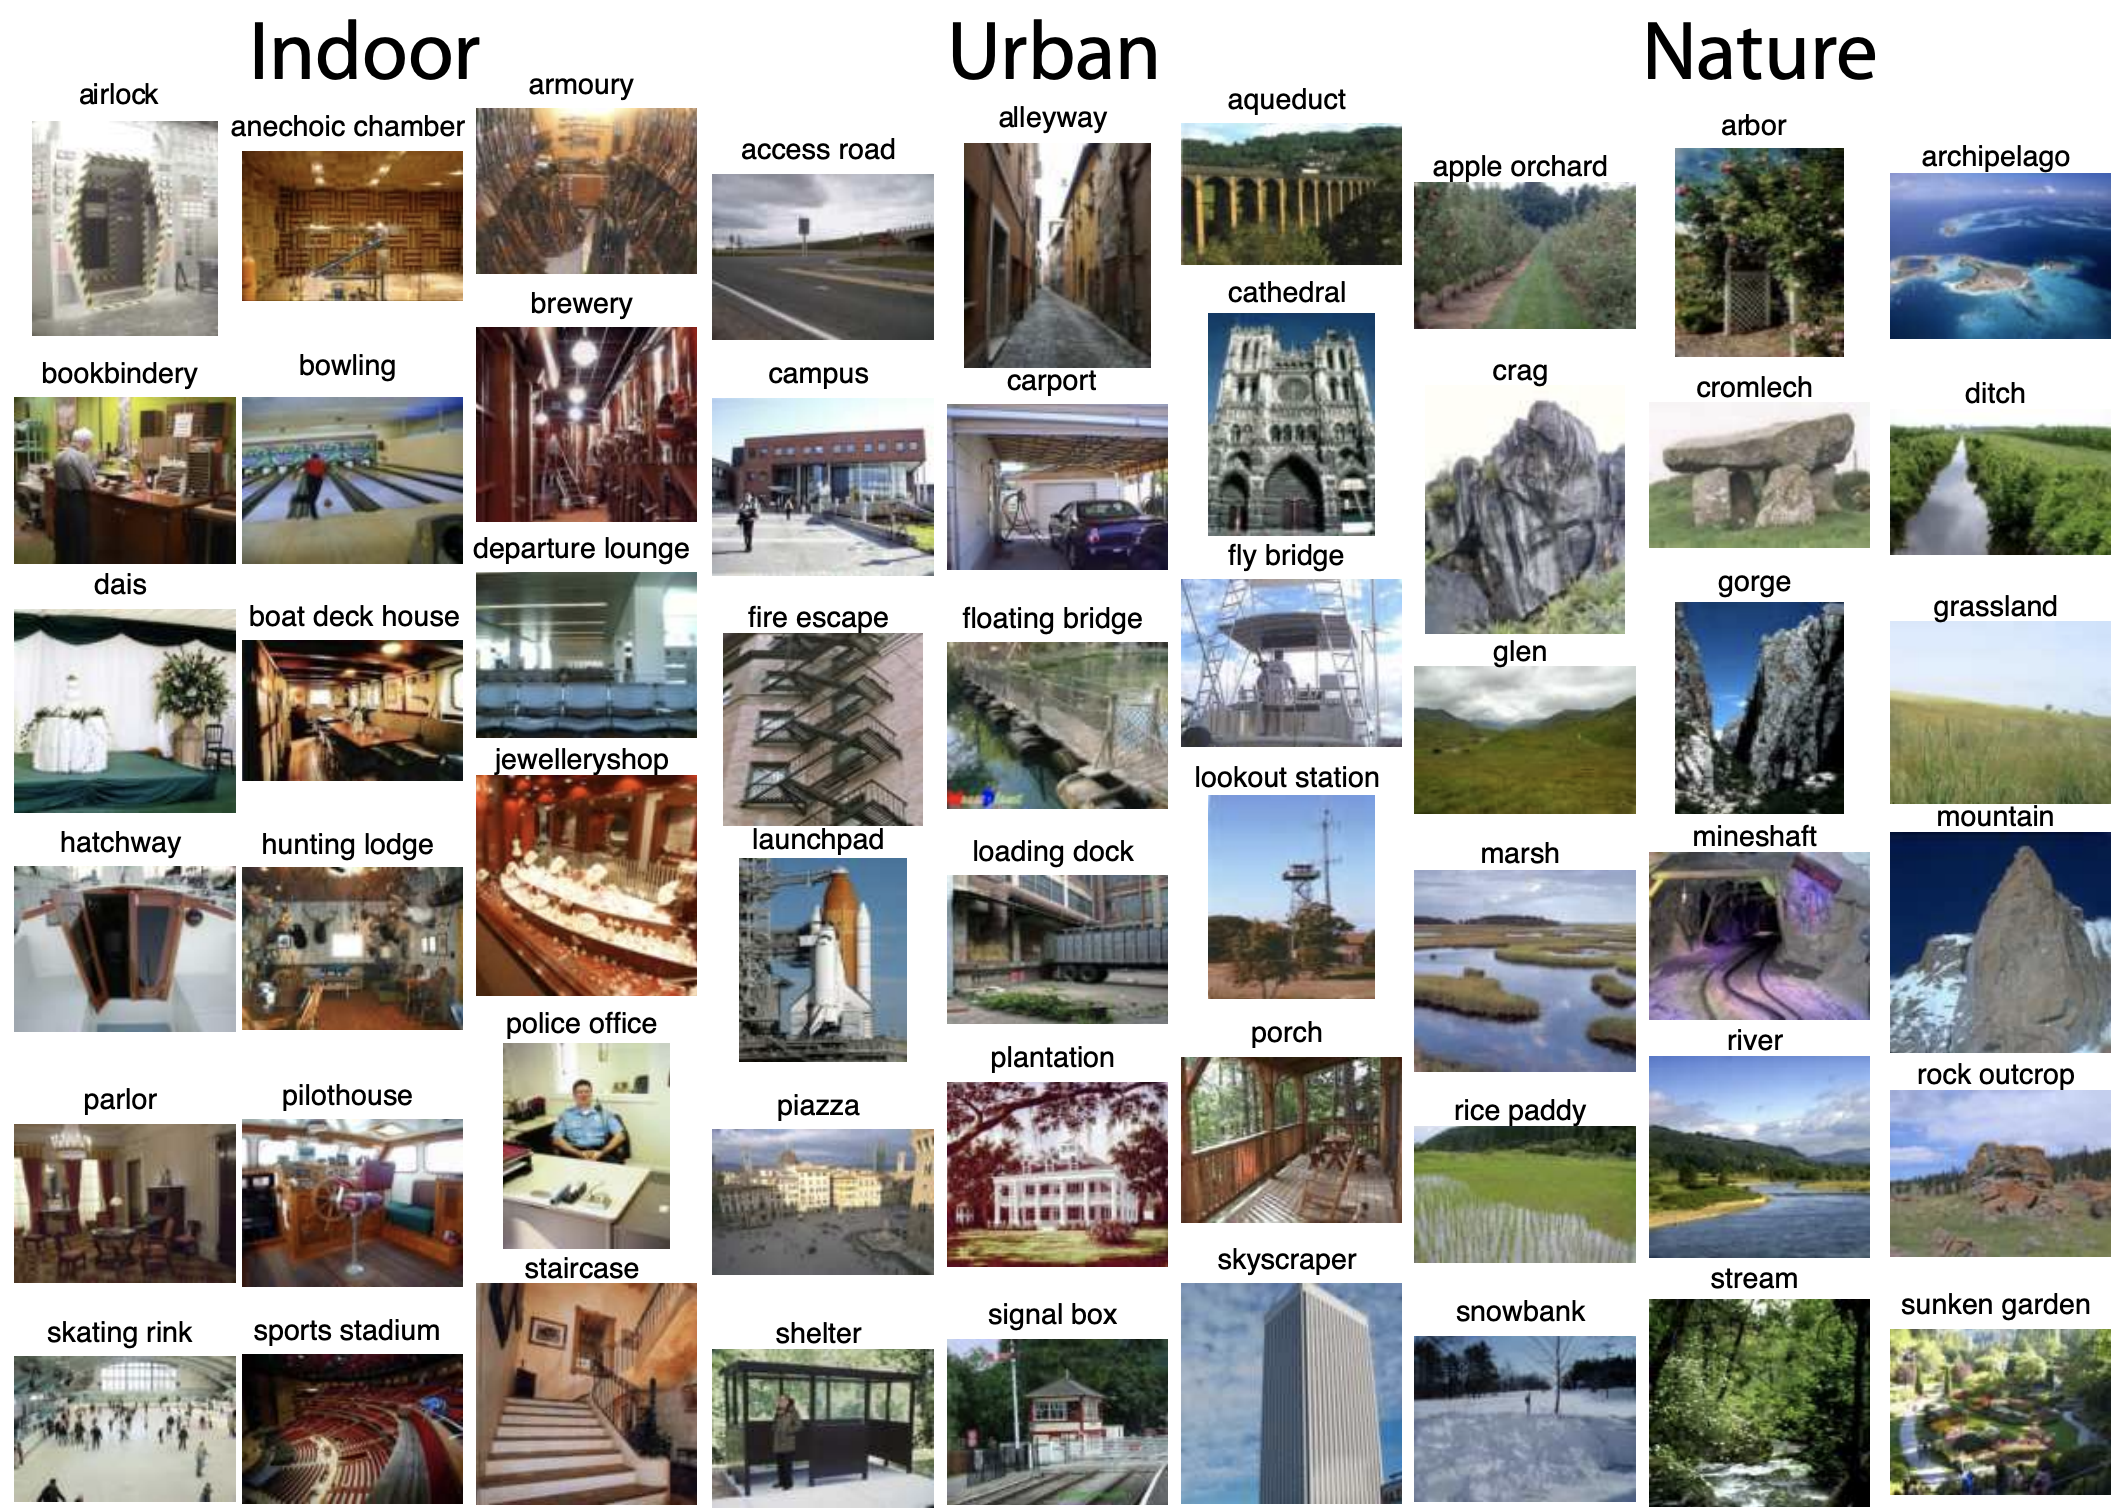
\includegraphics[width=0.95\linewidth]{Sun}
   	\end{center}
   	\caption{Примеры размеченных фотографий из датасета \textit{SUN}.}
   	\label{tikzpicture: sun}
\end{figure}

Ознакомиться с другими изображениями из датасета \textit{SUN} можно через 
интерактивный веб-обозреватель\footnote{groups.csail.mit.edu/vision/SUN/}, которым
можно воспользоваться для просмотра упорядоченных изображений как 
по сценам, так и по объектам.


\subsection{Адоптация датасета SUN}

\indent
\indent
Как было сказано во введении, названия локаций (сцен) из датасета \textit{SUN} не 
являются сами по себе популярными тегами из социальных сетей. Поэтому 
прежде всего необходимо выполнить сопоставление. Условно можно
разбить процедуру сопоставления на 2 части: объединение исходных классов 
датасета \textit{SUN} в семантические домены и сопоставление полученных доменов
с популярными хэштегами. В качестве источника хэштегов была выбрана социальная
сеть \textit{Instagram}\footnote{www.instagram.com}, ориентированная на обмен фото
и видео контентом между пользователями.

\indent
Итак, предварительно необходимо очистить названия классов \textit{SUN} от служебных
слов и символов, таких как \textit{indoor, outdoor, exterier, interier}, знаков "/" и 
однобуквенных алфавитных указателей. Затем для полученных слов или 
словосочетаний подбирается соответсвующий синсет из базы знаний \textit{Wordnet}.
Далее для синсетов находились гиперонимы, которые либо уже были достаточно
абстрактны, чтобы представлять собой часто встречающийся тег, либо 
автор работы находил для синсетов обобщающее понятие вручную.
Несколько примеров приведено в таблице~\ref{tabular: mapping}.


% Таблица о сопоставлении классов и тегов
\begin{table}[h]
    \begin{center}
        \begin{tabular}{c | c| c | c | c}
            \hline
            № & Исходное название & Синсет & Гипероним & Хэштег \\
            \hline
    
            1 & /s/shoe\_shop & shoe shop & shop & \htag{shopping} \\
    
            2 & /t/toyshop & toyshop & shop & \htag{shopping} \\
   
            3 & /v/volleyball\_court/indoor & volleyball court & court & \htag{sport} \\
    
            4 & /w/wrestling\_ring/indoor & wrestling ring & ring  & \htag{sport} \\
    
            5 & /r/rainforest & rain forest & forest & \htag{forest} \\
            
            6 & /p/pantry & pantry & storeroom & ? \\
   
            \hline
        \end{tabular}
    \end{center}
    \caption{Сопоставление искомых классов и хэштегов.}
    \label{tabular: mapping}
\end{table}


\indent
Из таблицы~\ref{tabular: mapping} видно, что некоторые синсеты имеют общие
гиперонимы. Кроме того, некоторые гиперонимы без каких-либо
дополнительных изменений могли быть использованы пользователями в качестве 
тегов. Таким образом, использование гиперонимов позволило немного уменьшить
количество ручной работы. Так же в таблице~\ref{tabular: mapping} приведен пример,
когда для локации сложно подобрать какой-то подходящий и широко распространенный
тег.  В итоге использовалось около половины из  \textit{397}
искомых классов датасета \textit{SUN}, каждому из которых удалось поставить
в соответсвие один из \textit{20} популярных хэштегов. В данной работе 
популярными считаются теги, использованные в сети
\textit{Instagram} более \textit{10 млн.} раз. При этом среднее число упоминаний 
отобранных тегов составило \textit{100 млн.} раз, а
максимальное --- \textit{450 млн.}. Полная информация о частоте встречаемости
для всех хэштегов приведена на рисунке ~\ref{tikzpicture: tags_counts}.


% Гистограмма встречаемости хэштегов
\begin{center}
    \begin{figure}[h]
    \begin{tikzpicture}
    \label{tags_counts}
        \begin{axis}[
            ylabel = Число использований млн.,
            x tick label style={rotate=90,anchor=east},
            width = 0.7\paperwidth,
            height = 0.4\paperheight,
            symbolic x coords=
            {
                art,
                nature,
                beach,
                sky,
                home,
                shopping,
                artchitecture,
                water,
                sport,
                street,
                car,
                cafe,
                garden,
                urban,
                forest,
                bar,
                church,
                building,
                road,
                airport,
                entertainment,
                science
            },
            xtick=data
          ]
            \addplot[ybar,fill=blue] coordinates {
                (art, 450)
                (nature, 390)
                (beach, 210)
                (sky, 190)
                (home, 115)
                (shopping, 100)
                (artchitecture, 97)
                (water, 65)
                (sport, 60)
                (street, 55)
                (car, 55)
                (cafe, 45)
                (garden, 41)
                (urban, 32)
                (forest, 30)
                (bar, 25)
                (church, 25)
                (building, 23)
                (road, 17)
                (airport, 14)
                (entertainment, 10)
                (science, 10)
            };
        \end{axis}
    \end{tikzpicture}
    \caption{Встречаемость предсказываемых хэштегов в социальной сети \textit{Instagram}.}
    \label{tikzpicture: tags_counts}
    \end{figure}
\end{center}


\indent 
Отметим, что автор предпринял несколько попыток произвести процедуру 
адаптации разметки датасета \textit{SUN} полностью автоматически, 
но они оказались неудачными. 


\indent
\indent
Первая попытка --- обобщить искомые классы, используя метод \textit{topic\_domains},
который доступен для синсетов в \textit{python} реализации API к 
базе \textit{WordNet}. Например, для синсета
\textit{basketball\_court.n.01}, который определяется как 
\textit{the court on which basketball is played}, 
вызов данного метода возвращает \textit{basketball.n.02}, который определяется так:
\textit{a game played on a court by two opposing teams of 5 players;
points are scored by throwing the ball through an elevated horizontal hoop}.
К сожалению, проблема заключалась в том, что для подавляющего числа названий 
локаций \textit{topic\_domains} возвращал пустое значение, т.е. для этих синсетов
авторами базы знаний не было назначено доменов.


\indent
\indent
Вторая попытка аналогичная первой, но использовалась сторонняя база знаний
\textit{WordNet Domains}\footnote{http://wndomains.fbk.eu/}. К сожалению, такое
расширение базы доменов не позволило решить проблему, описанную выше.


\indent
\indent
Третья идея заключась в использовании информации о семантической близости 
синсетов, в частности, API \textit{WordNet'a} позволяет для любых двух синсетов
вычислить степень похожести несколькими способами:
\textit{jcn\_similarity, lch\_similarity, res\_similarity, wup\_similarity}.
Для разных видов измерения расстояния были вычислены матрицы попарных дистанций,
на основе которых производилась иерархическая кластеризация с различными
гиперпараметрами
 (например, класторизация по заданному максимальному расстоянию в кластере, 
по заданному количеству кластеров). К сожалению, автору не удалось получить кластеры,
большую часть которых можно было бы без труда "озаглавить" 
каким-либо популярным хэштегом.


\indent
\indent
Таким образом, процедуру сопоставления всех 
\textit{397} искомых классов датасета \textit{SUN} и хэштегов из социальной сети \textit{Instagram}
пришлось произвести в полуручном режиме (опираясь только на гиперонимы),
как это было описано выше в данном разделе.


\indent
\indent
Приведем пример такого сопостовления. В таблице \ref{tabular: sport_classes} 
перечислены названия локаций, которым поставлен в соответсвие хэштег \htag{sport}:

\begin{table}[ht!]
    \begin{center}
        \begin{tabular}{c | c | c}
            /w/wrestling\_ring/indoor &
            /a/athletic\_field/outdoor &
            /b/badminton\_court/indoor
            \\
            /b/ball\_pit &
            /b/baseball\_field &
            /b/basketball\_court/outdoor
            \\
            /b/boxing\_ring &
            /b/bullring &
            /g/golf\_course
            \\
            /g/gymnasium/indoor &
            /m/martial\_arts\_gym &
            /r/racecourse
            \\
            /r/riding\_arena &
            /s/ski\_lodge &
            /s/ski\_resort
            \\
            /s/ski\_slope &
            /s/squash\_court &
            /s/stadium/baseball
            \\
            /s/stadium/football &
            /s/swimming\_pool/indoor &
            /s/swimming\_pool/outdoor
            \\
            /t/tennis\_court/indoor &
            /t/tennis\_court/outdoor &
            /v/volleyball\_court/indoor
            \\
            /v/volleyball\_court/outdoor          
        \end{tabular}
    \end{center}
    \caption{Список классов датасета \textit{SUN}, которым сопоставлен хэштег \htag{sport}.}
    \label{tabular: sport_classes}
\end{table}

Файлы с полной информацией об итоговом сопоставлении можно найти в 
репозитории автора\footnote{github.com/AlekseySh/scenes}.


\newpage
\section{Численные эксперименты}

\subsection{Архитектура программы}

\subsection{Особенности реализации}

\subsection{Полученные результаты}

\subsection{Обсуждение результатов}


\newpage
\section{Валидация результатов}


\newpage
\section*{Выводы}
\addcontentsline{toc}{section}{\tocsecindent{Выводы}}


\newpage
\addcontentsline{toc}{section}{\tocsecindent{Список литературы}}
\begin{thebibliography}{99}

	\bigskip
	
	\bibitem{imagenet}
	Olga Russakovsky, Jia Deng, Hao Su, Jonathan Krause, Sanjeev Satheesh, 
	Sean Ma, Zhiheng Huang, Andrej Karpathy, Aditya Khosla, Michael Bernstein, 
	Alexander C. Berg and Li Fei-Fei. [2015] \textit{ImageNet Large Scale
	 Visual Recognition Challenge}. IJCV.
	 % http://ai.stanford.edu/~olga/bibtex/ILSVRC15.bib
	 
	 
	
\end{thebibliography}


\end{document} 
